\documentclass[tikz,border=5]{standalone}
\usepackage{circuitikz}
  \tikzset{wind/.style={line width = 1pt, color=white, fill=black, line join=round}}
\begin{document} 
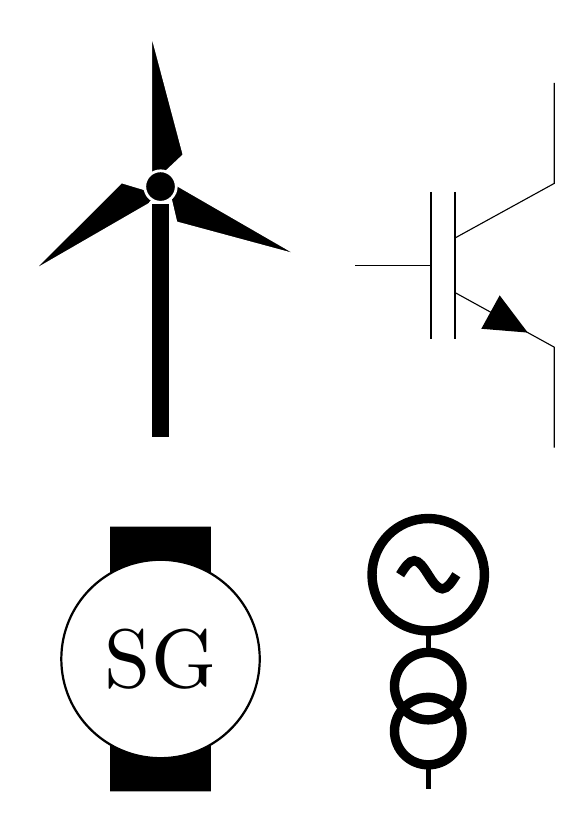
\begin{tikzpicture}
\foreach \i in {90, 210, 330}{
    \draw [wind, rotate=\i] 
      (0,0.125) -- (2,0.125) -- (2,0.125) -- (0.4,-0.3) -- cycle;
}
\draw[wind] (0,0) circle [radius=.2];
\draw[wind] (-0.125, -0.2) rectangle ++(0.25, -3);
\node[nigbt, scale=3] at (5, -1) {};
\node[elmech, scale=3] at (0, -6) {SG};
\scalebox{1.7}{\draw[line width = 1pt, color=black] (2, -2.5) to[sinusoidal voltage source] (2, -3.3) to[oosourcetrans] (2, -4.5);}
\end{tikzpicture}
\end{document}